\documentclass{standalone}
\usepackage{tikz}

\begin{document}
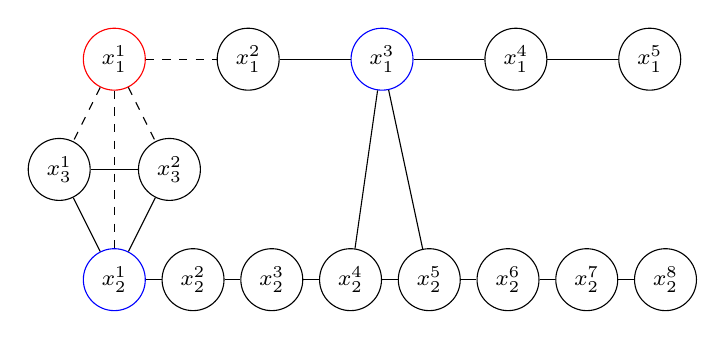
\begin{tikzpicture}
    \node[circle, minimum width =10pt , minimum height =10pt ,draw= red] (1) at(0,2){\begin{footnotesize}$x_1^1$\end{footnotesize}};
    \node[circle, minimum width =10pt , minimum height =10pt ,draw=black] (2) at(1.7,2){\begin{footnotesize}$x_1^2$\end{footnotesize}};
    \node[circle, minimum width =10pt , minimum height =10pt ,draw=blue] (3) at(3.4,2){\begin{footnotesize}$x_1^3$\end{footnotesize}};
    \node[circle, minimum width =10pt , minimum height =10pt ,draw=black] (4) at(5.1,2){\begin{footnotesize}$x_1^4$\end{footnotesize}};
    \node[circle, minimum width =10pt , minimum height =10pt ,draw=black] (5) at(6.8,2){\begin{footnotesize}$x_1^5$\end{footnotesize}};
    \node[circle, minimum width =10pt , minimum height =10pt ,draw=black] (6) at(-0.7,0.6){\begin{footnotesize}$x_3^1$\end{footnotesize}};
    \node[circle, minimum width =10pt , minimum height =10pt ,draw=black] (7) at(0.7,0.6){\begin{footnotesize}$x_3^2$\end{footnotesize}};
    \node[circle, minimum width =10pt , minimum height =10pt ,draw=blue] (8) at(0,-0.8){\begin{footnotesize}$x_2^1$\end{footnotesize}};
    \node[circle, minimum width =10pt , minimum height =10pt ,draw=black] (9) at(1,-0.8){\begin{footnotesize}$x_2^2$\end{footnotesize}};
    \node[circle, minimum width =10pt , minimum height =10pt ,draw=black] (10) at(2,-0.8){\begin{footnotesize}$x_2^3$\end{footnotesize}};
    \node[circle, minimum width =10pt , minimum height =10pt ,draw=black] (11) at(3,-0.8){\begin{footnotesize}$x_2^4$\end{footnotesize}};
    \node[circle, minimum width =10pt , minimum height =10pt ,draw=black] (12) at(4,-0.8){\begin{footnotesize}$x_2^5$\end{footnotesize}};
    \node[circle, minimum width =10pt , minimum height =10pt ,draw=black] (13) at(5,-0.8){\begin{footnotesize}$x_2^6$\end{footnotesize}};
    \node[circle, minimum width =10pt , minimum height =10pt ,draw=black] (14) at(6,-0.8){\begin{footnotesize}$x_2^7$\end{footnotesize}};
    \node[circle, minimum width =10pt , minimum height =10pt ,draw=black] (15) at(7,-0.8){\begin{footnotesize}$x_2^8$\end{footnotesize}};
    \draw[dashed] (1) --(2);
    \draw[-] (2)--(3) --(4)--(5);
    \draw[-] (6)--(7);
    \draw[-] (8)--(9)--(10)--(11)--(12)--(13)--(14)--(15);
    \draw[dashed] (1)--(6)  (1)--(7);
    \draw[-] (8)--(6)  (8)--(7);
    \draw[-] (3)--(11)  (3)--(12);
    \draw[dashed] (1)--(8);
    
    \end{tikzpicture}
\end{document}